


We limit our investigation of the total amount of testing being conducted to the last 39 months from January 2013 to March 2016.

\includegraphics{Figures/Monthly-TSPlot}


There is a (perhaps not so obvious) pattern in this data to draw to the reader's attention. It seems both a seasonal effect over the months within a year, and a general increase over years should be noted.  Our belief in this notion is supported by use of an Analysis of Variance (ANOVA) procedure.


\begin{Schunk}
\begin{Soutput}
Analysis of Variance Table

Response: n
                 Df  Sum Sq Mean Sq F value    Pr(>F)    
as.numeric(Year)  1 4961349 4961349 54.1576 1.339e-07 ***
Year              2  223442  111721  1.2195 0.3130261    
Month            11 5773449  524859  5.7293 0.0001773 ***
Residuals        24 2198628   91609                      
---
Signif. codes:  0 '***' 0.001 '**' 0.01 '*' 0.05 '.' 0.1 ' ' 1
\end{Soutput}
\end{Schunk}



The above table shows that the impact of year can be summarised as a straight line effect, while we have a cyclic pattern over the months. Any departure from this would constitute an unusual increase in total workload since the introduction of RenalQ. We use a standard control chart for individuals to search for unusual results. The control limits on the plot are calculated using the data from before the introduction of RenalQ and are at two (shown in orange) and three (shown in red) standard deviations from the centre line.

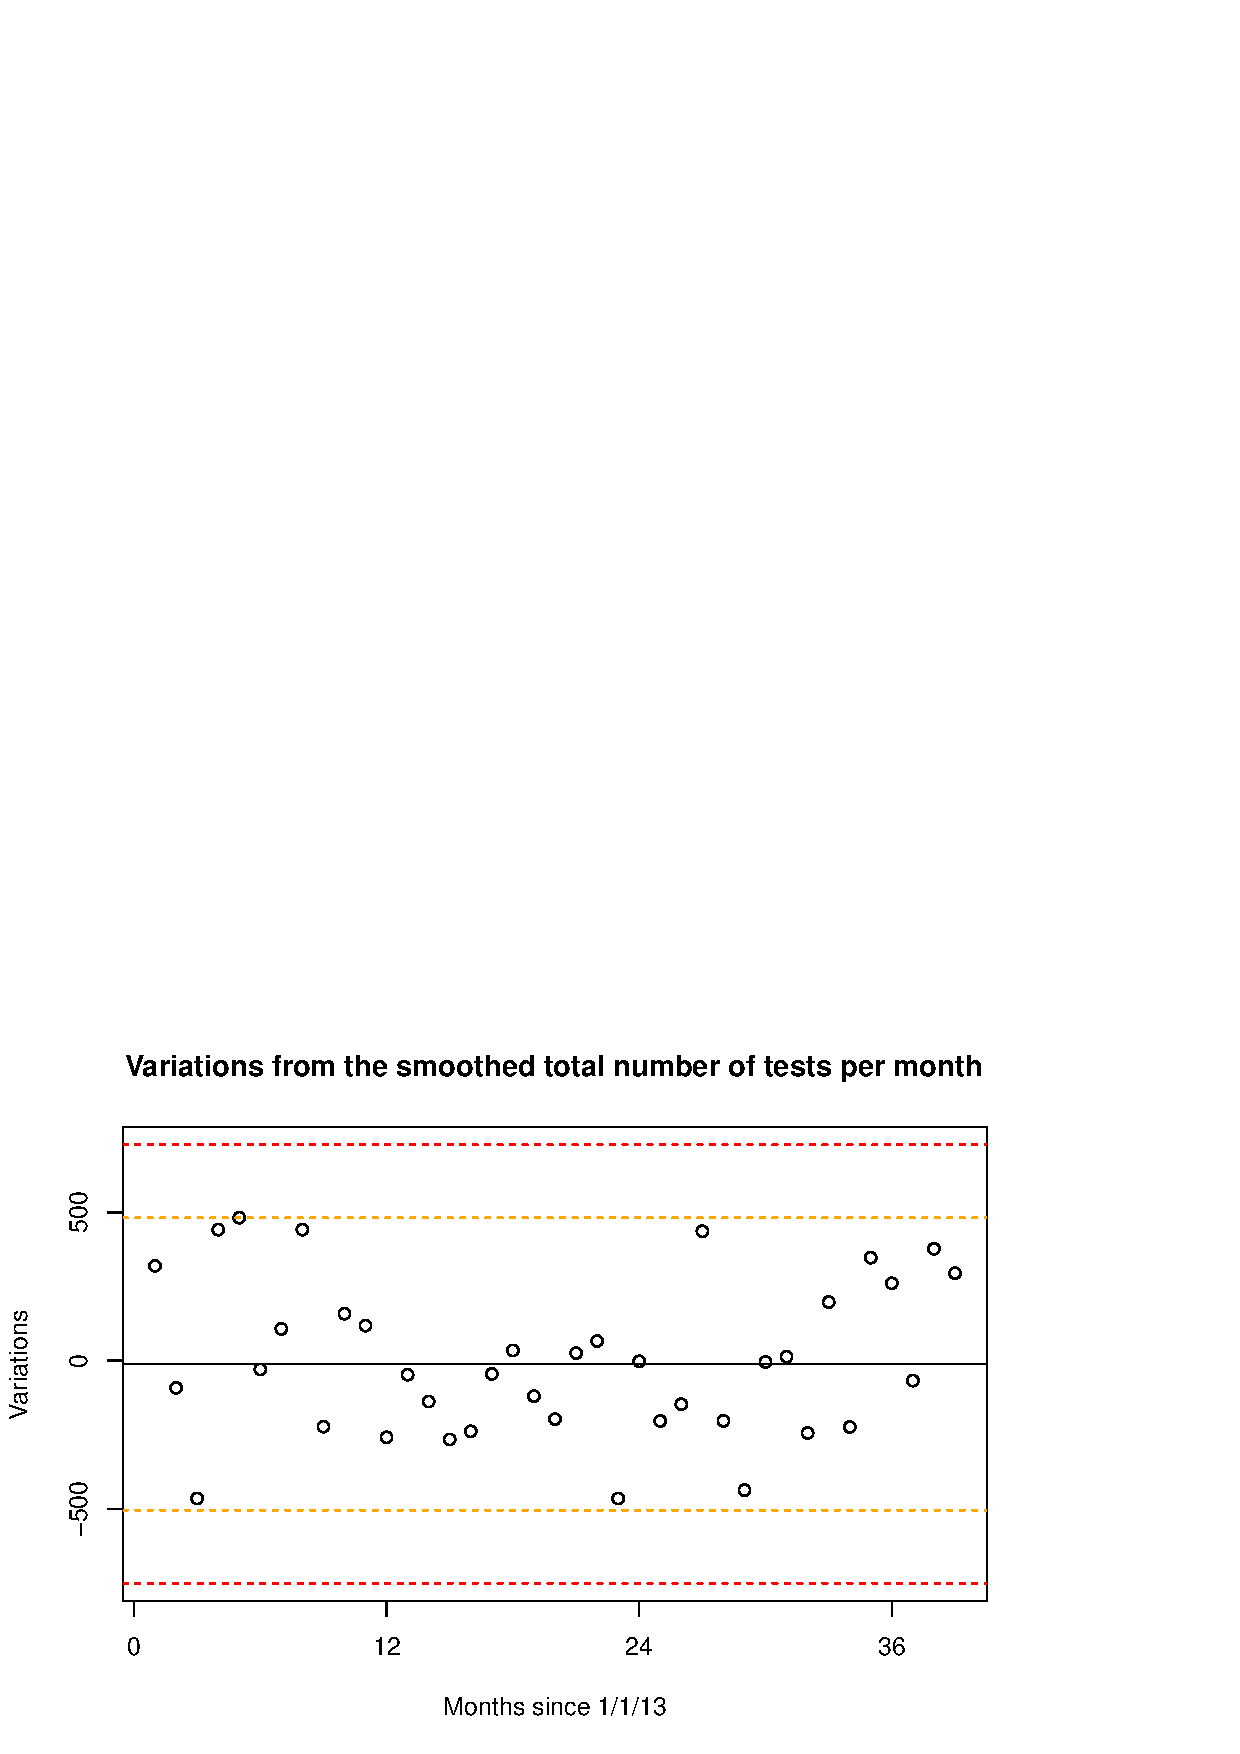
\includegraphics{Figures/Monthly-QCC}

There are no serious  departures (outside three standard deviation limits) from what could be expected in terms of the total number of tests being conducted. We do need to condition this assessment on our concern that the totality of tests has not been provided for earlier years of this investigation. This aspect of this report can be re-created once the reliability of the complete data can be established.

